% Modified from Fig 2.1 in Xiang Sun's notes.
\documentclass[tikz,border=2pt]{standalone}
\usetikzlibrary{arrows.meta,positioning}

\usepackage{anyfontsize} % allows arbitrary font sizes
\usepackage{lmodern} % better font scaling

\makeatletter
\renewcommand\normalsize{%
  \@setfontsize\normalsize{16pt}{19pt}%
}
\renewcommand\Large{%
  \@setfontsize\Large{20pt}{24pt}%
}
\makeatother

\begin{document}
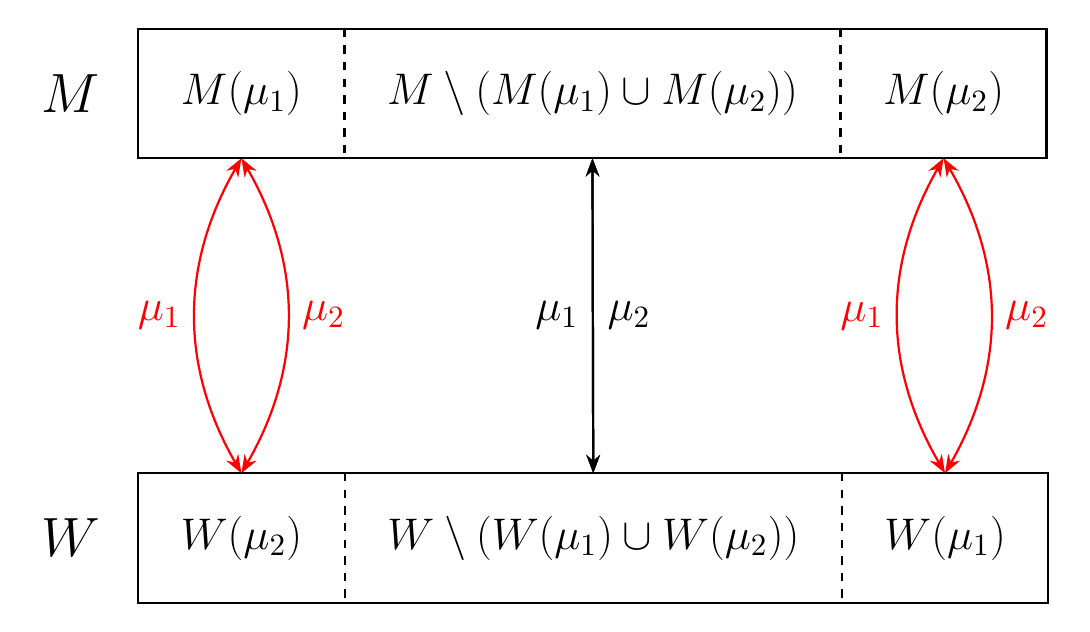
\begin{tikzpicture}[thick,box/.style={rectangle,inner sep=15pt,align=center},>=Stealth]

% Top row: M
\node[box] (M1) {$M(\mu_1)$};
\node[box,right=0pt of M1] (Mmid) {$M \setminus (M(\mu_1)\cup M(\mu_2))$};
\node[box,right=0pt of Mmid] (M2) {$M(\mu_2)$};

% Bottom row: W
\node[box,below=4cm of M1] (W1) {$W(\mu_2)$};
\node[box,right=0pt of W1] (Wmid) {$W \setminus (W(\mu_1)\cup W(\mu_2))$};
\node[box,right=0pt of Wmid] (W2) {$W(\mu_1)$};

% Labels on left
\node[left=0.3cm of M1] {\Large $M$};
\node[left=0.3cm of W1] {\Large $W$};

% Vertical arrows (black) middle
\draw[<->] (Mmid.south) -- node[left] {$\mu_1$} (Wmid.north);
\draw[<->] (Wmid.north) -- node[right] {$\mu_2$} (Mmid.south);

% Red curved arrows left
\draw[red,<->,bend left=30] (W1.north) to node[left] {$\mu_1$} (M1.south);
\draw[red,<->,bend left=30] (M1.south) to node[right] {$\mu_2$} (W1.north);

% Red curved arrows right
\draw[red,<->,bend left=30] (W2.north) to node[left] {$\mu_1$} (M2.south);
\draw[red,<->,bend left=30] (M2.south) to node[right] {$\mu_2$} (W2.north);

% Dashed separators
\draw[dashed] (Mmid.north west) -- (Mmid.south west);
\draw[dashed] (Mmid.north east) -- (Mmid.south east);
\draw[dashed] (Wmid.north west) -- (Wmid.south west);
\draw[dashed] (Wmid.north east) -- (Wmid.south east);

% Outer boxes.
\draw (M1.north west) -- (M2.north east) -- (M2.south east) -- (M1.south west) -- cycle;
\draw (W1.north west) -- (W2.north east) -- (W2.south east) -- (W1.south west) -- cycle;

\end{tikzpicture}
\end{document}
